\documentclass[tikz,border=2pt]{standalone}
\usepackage{amsmath}
\usepackage{pgfplots}
\pgfplotsset{compat=1.18}
\usetikzlibrary{arrows.meta}
\begin{document}
% Property 2.4, Example 2: V=[0,2]x[0,1], p=(3,-2), nearest point q=(2,0), p-q=(1,-2), dist=sqrt(5).
% Angle condition: for x=(1,1) in V, (p-q)^T(x-q)=(1,-2)^T(-1,1)=-3<=0, the angle is obtuse;
% supporting hyperplane H={x1-2x2=2} through q with normal p-q meets V only at q.
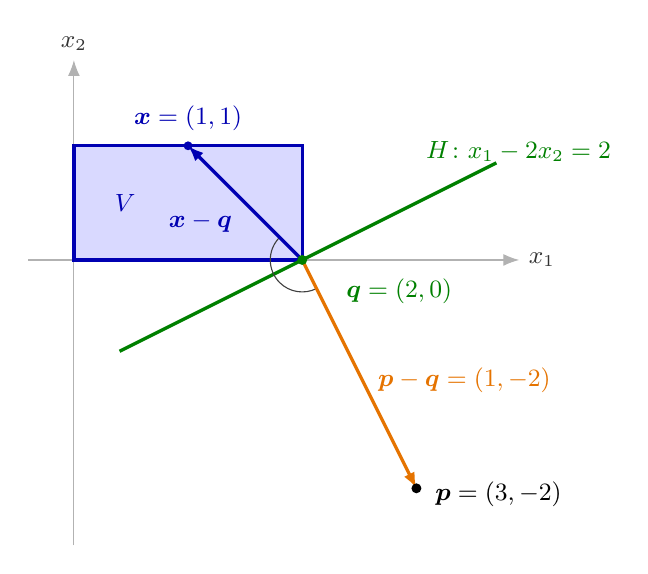
\begin{tikzpicture}[font=\small, >={Latex[length=2mm]}, x=1.45cm, y=1.45cm]
  % axes
  \draw[gray!60, ->] (-0.4,0) -- (3.9,0) node[anchor=west, gray!40!black] {$x_1$};
  \draw[gray!60, ->] (0,-2.5) -- (0,1.75) node[anchor=south, gray!40!black] {$x_2$};
  % V = [0,2] x [0,1]
  \fill[blue!15] (0,0) rectangle (2,1);
  \draw[blue!70!black, very thick] (0,0) rectangle (2,1);
  \node[blue!70!black] at (0.45,0.5) {$V$};
  % supporting hyperplane H: x1-2x2=2
  \draw[green!50!black, very thick] (0.4,-0.8) -- (3.7,0.85);
  \node[green!50!black, anchor=west] at (3.0,0.95) {$H\colon x_1-2x_2=2$};
  % angle between p-q and x-q (about 162 degrees)
  \draw[gray!50!black] (2,0) ++(135:0.28) arc (135:296.57:0.28);
  % vectors
  \draw[blue!70!black, very thick, ->] (2,0) -- (1,1);
  \draw[orange!90!black, very thick, ->] (2,0) -- (3,-2);
  \node[orange!90!black, anchor=west] at (2.58,-1.05) {$\boldsymbol{p}-\boldsymbol{q}=(1,-2)$};
  \node[blue!70!black, anchor=north east] at (1.47,0.5) {$\boldsymbol{x}-\boldsymbol{q}$};
  % points
  \fill[black] (3,-2) circle (1.8pt);
  \node[anchor=west] at (3.08,-2.05) {$\boldsymbol{p}=(3,-2)$};
  \fill[green!50!black] (2,0) circle (1.8pt);
  \node[green!50!black, anchor=north west] at (2.3,-0.08) {$\boldsymbol{q}=(2,0)$};
  \fill[blue!70!black] (1,1) circle (1.6pt);
  \node[blue!70!black, anchor=south] at (1,1.05) {$\boldsymbol{x}=(1,1)$};
\end{tikzpicture}
\end{document}
